\documentclass[aspectratio=169,handout, 10pt]{beamer}
\usepackage[utf8]{inputenc}

% packages
\usepackage{color}
\usepackage{graphicx}
\usepackage{adjustbox}
\usepackage{amsmath, amsfonts, amssymb, bm}
\usepackage{natbib}
%\usepackage{enumitem}
\usepackage{longtable}
\usepackage{multicol}
\usepackage{siunitx} %%% <<<<< THIS PACKAGE WAS MISSING LEADING TO ERRORS in \num{}
%% Graph
\usepackage{transparent}
\usepackage{subcaption}
\usepackage{sidecap}
\usepackage{tikz}
\usetikzlibrary{shapes.geometric, positioning, arrows.meta}
\usepackage{circuitikz}

\usepackage{adjustbox}

\setbeamertemplate{navigation symbols}{}
\setbeamertemplate{headline}{}
\setbeamertemplate{footline}












% Packages
\usepackage{geometry}
\usepackage{graphicx}
\usepackage{amsmath, amsfonts, amssymb, bm}

\usepackage{adjustbox}
\usepackage{transparent}
\usepackage{subcaption}
\usepackage{sidecap}
\usepackage{tikz}
\usetikzlibrary{shapes.geometric, positioning, arrows.meta}
\usepackage{circuitikz}
\usepackage{tikz}
%\usepackage{fancyhdr}
\usepackage{appendixnumberbeamer}
\usepackage[labelformat=empty]{caption}




\usepackage{adjustbox}

\setbeamertemplate{navigation symbols}{}
\setbeamertemplate{headline}{}
\setbeamertemplate{footline}{\insertframenumber/\inserttotalframenumber}
\usepackage{appendixnumberbeamer}
%\usepackage[labelformat=empty]{caption}


\graphicspath{{Figures and Tables/}}

\begin{document}
\newgeometry{margin = 0pt}
%%%%%%%%%%%%%%%%%%%%%%%%%%%%%%%%%%%%%%%%%%%%%%%%%%%%%%%%%%%%%%
% Slide 1: Title Page

\begin{frame}[noframenumbering,plain]
\vspace{9pt}
  \begin{figure}
\fullframegraphic{
\includegraphics[width= \paperwidth, height = \paperheight]{Front Page.pdf}}
       \end{figure}
\end{frame}

%%%%%%%%%%%%%%%%%%%%%%%%%%%%%%%%%%%%%%%%%%%%%%%%%%%%%%%%%%%%
\restoregeometry
%\begin{frame}%[noframenumbering,plain]
%    \titlepage
%\end{frame}

% Remove background image for subsequent slides
%\usebackgroundtemplate{}
%	\titlepage
%	\textbf{Supervisors}: Prof. Axel Weber (First); Prof.  
 %                             Krystof Hegemejer (Second)
%\end{frame}
%%%%%%%%%%%%%%%%%%%%%%%%%%%%%%%%%%%%%%%%%%%%%%%%%%%%%%%%%%%%%%%%%

\begin{frame}{Chapter One: Introduction}
        \begin{itemize}
    \item Centrality of health outcome to economic but global development: Post-Covid 19
    \item Social protection relevance to UHC (Systematic review in Yakobori et al. 2023), with two major achievements:
    \begin{enumerate}[i]
        \item Right approach in public health discourse, i.e. SP floor, ADB SP index
        \item Health financing models: Social security and social assistance
    \end{enumerate}
    \item Insufficiency of health investment capital created the demand for ODA in developing countries: 0.7\% of GNI endorsed in 1970 at the United Nations development decades and 2002 Monterrey Consensus on development financing in Mexico
    \begin{enumerate}[i]
        \item Aid Effectiveness Debate: Optimists vs. Pessimists
        \item Conditional and non-linearity of ODA Effectiveness
    \end{enumerate}
    \item Gaps in the past studies
    \begin{enumerate}[i]
        \item Choice of predictor: Total vs Health ODA; Commitment vs Disbursement 
        \item Lack of comprehensive outcome indicators endangers cross-country comparison 
        \item More importantly, mechanism of the effect of ODA on Health outcome
        \item Methodological problem 
    \end{enumerate}
\end{itemize}
\end{frame}


\begin{frame}{Introduction cont.}
\paragraph{\textbf{Primary Research Question:}}
\begin{itemize*}
    \item What is the overall effectiveness and impact of foreign aid, specifically Official Development Assistance (ODA), on health outcomes in developing countries? This overarching research question aims to investigate the comprehensive impact of ODA on diverse composite health dimensions created from relevant SDG 2 and 3 indicators.\\  
\end{itemize*}
\paragraph{\textbf{Sub Questions:}}
    \begin{enumerate}[i]
        \item What is the direct impact of ODA on health outcomes in developing countries?
        \item Are there regional variations in the impact of ODA on health outcomes, particularly in SSA and non-SSA regions?
        \item Is the impact of ODA on health outcomes mediated by social protection development in developing nations?
    \end{enumerate}

\end{frame}


%%%%%%%%%%%%%%%%%%%%%%%%%%%%%%%%%%%%%%%%%%%%%%%%%%%%%%%%%%%%%%%%%%

\begin{frame}{Chapter Two: Conceptual Clarification and Preliminary Analysis}
The chapter presents conceptual analysis of the three germane concepts in the study: foreign aid (ODA), health outcomes, and social protection, divided into two sections: 

\begin{itemize}
    \item Conceptual Clarification:
    \begin{itemize}
        \item ODA classification systems and method of data compilation
        \item Broadening the concept of health outcomes, moving from narrow health metrics to six composite health dimensions
        \item Highlights the complexity of social protection definition and metrics. Also lack of panel data for social protection. 
    \end{itemize}
    \item Characterization of respective variables' data
    \begin{itemize}
        \item Note: Preliminary data for ODA spans between 1990 to 2021, while the rest of the analysis only use data between 2000 to 2021 due to high missing values. 
    \end{itemize}
\end{itemize}
\end{frame}


%%%%%%%%%%%%%%%%%%%%%%%%%%%%%%%%%%%%%%%%%%%%%%%%%%%%%%%

\begin{frame}{Conceptual Analysis Cont.}
\textbf{Characterisation of ODA by Status and Sectors}\\
Note: All ODA are in 2021 constant price in USD billion, sourced from the OECD (2023)
\begin{columns}
      \column{0.47\textwidth}

            \begin{figure}
            \caption{Figure 1: Evolution of Disbursements and Commitments ODA}
            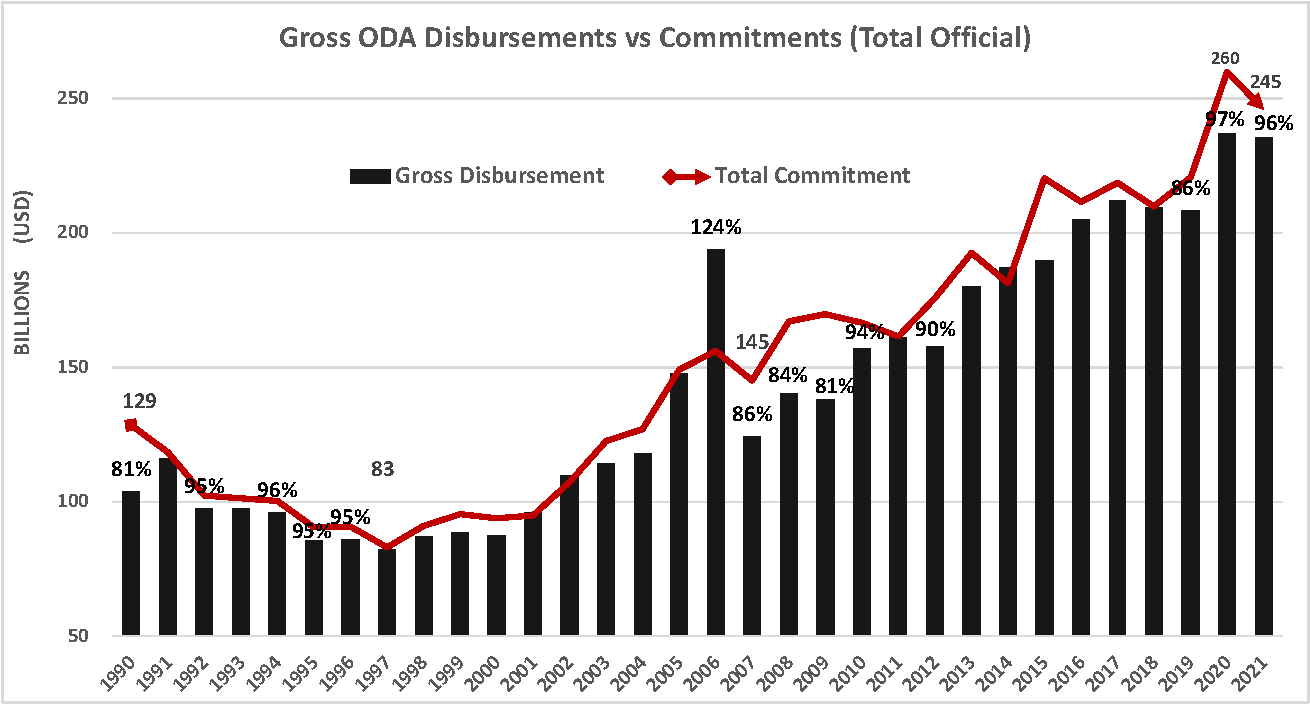
\includegraphics[width = \textwidth]{Figures and Tables/Dibs_VS_Commit.pdf}
        \end{figure}


\column{0.47\textwidth}
   \begin{figure}
   \caption{Figure 2: ODA Commitments of Sectors}
            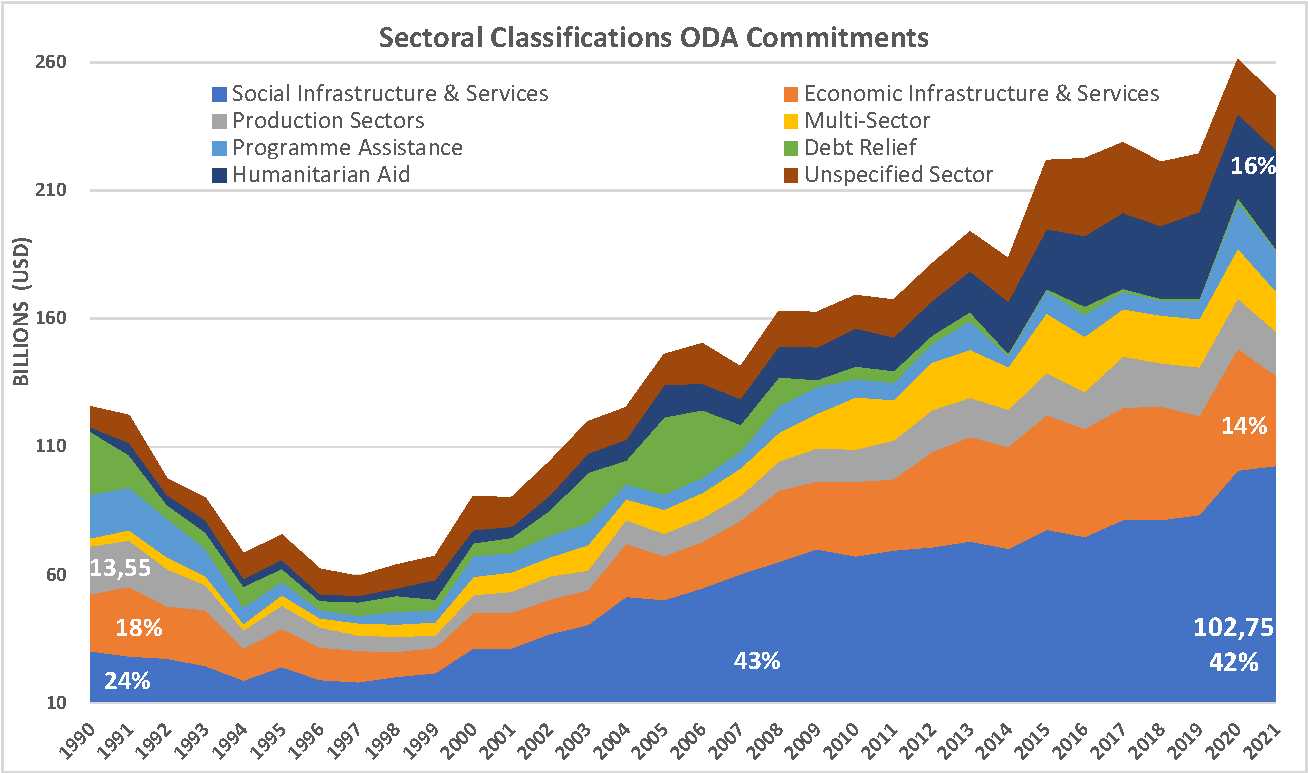
\includegraphics[width=\textwidth]{Figures and Tables/Sector_class.pdf}
            
        \end{figure}

        
    \end{columns}
\footnotesize{Note. Data for sectoral allocation of ODA is only available for commitment, and not disbursement. However, given the closeness of the two, commitment is a valid proxy for disbursement.}
\end{frame}


%%%%%%%%%%%%%%%%%%%%%%%%%%%%%%%%%%%%%%%%%%%%
\begin{frame}{Conceptual Analysis Cont.: ODA by Payment Status and Sectors}

\begin{columns}
      \column{0.47\textwidth}

            \begin{figure}
            \caption{Figure 3: Social Infrastructure Sector ODA}
            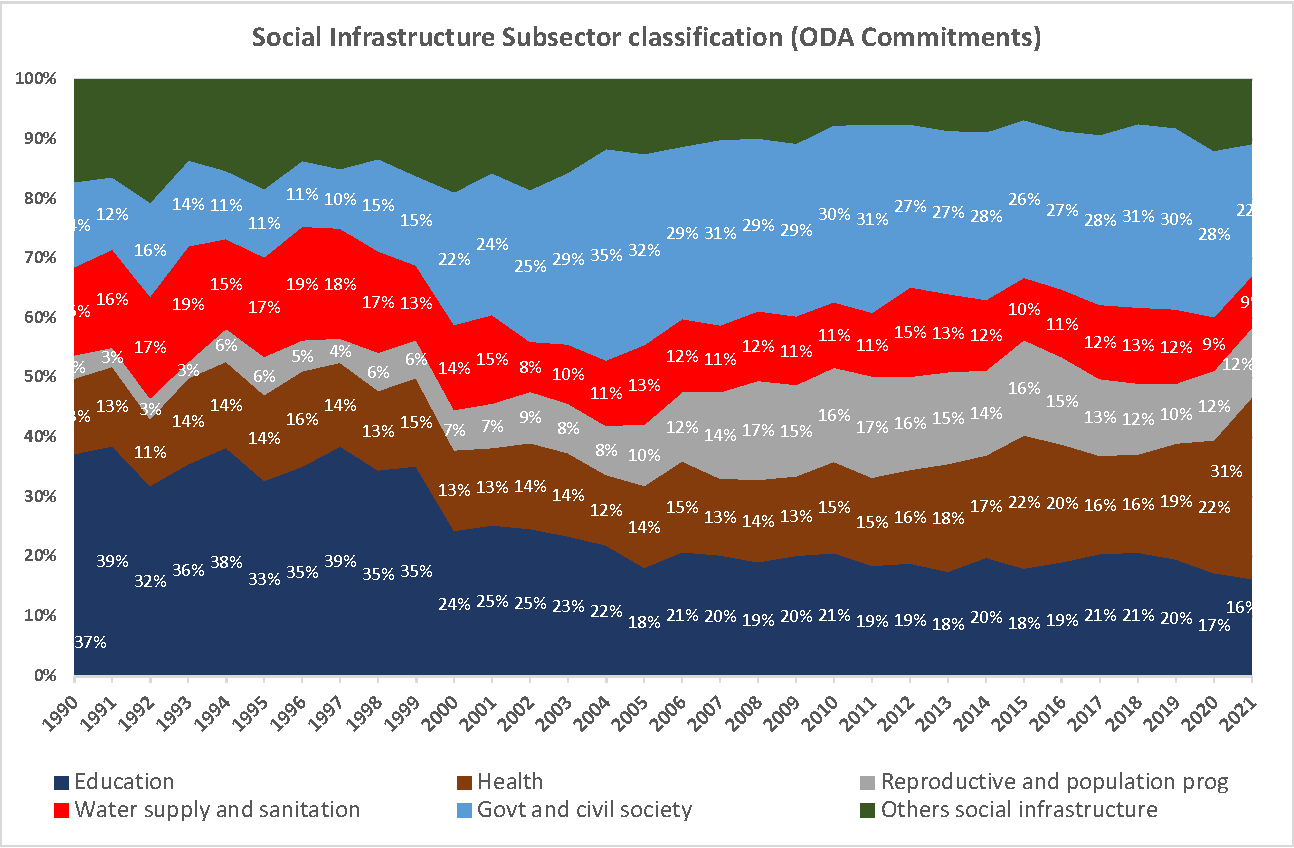
\includegraphics[width = \textwidth]{Figures and Tables/Subsectors_soc_inf.pdf}
        \end{figure}


\column{0.47\textwidth}
   \begin{figure}
   \caption{Figure 4: Donors' Classification of Net ODA}
            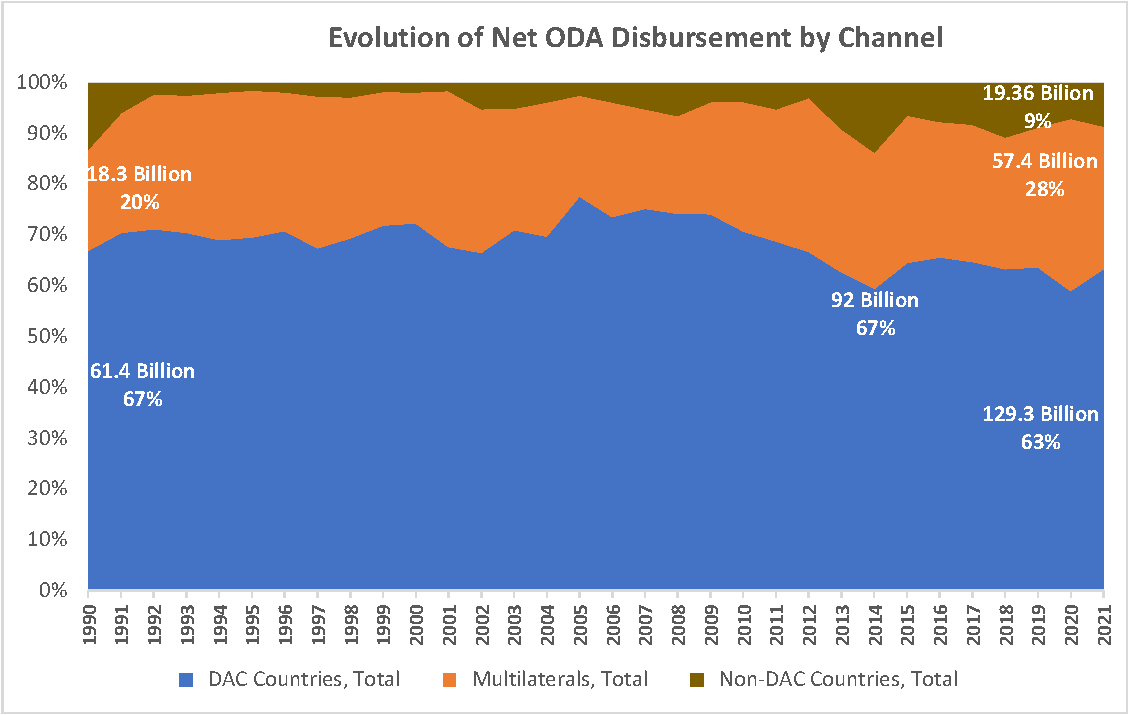
\includegraphics[width=\textwidth]{Figures and Tables/Evolution_Net_ODA.pdf}
            
        \end{figure}

        
    \end{columns}
\footnotesize{Despite growth in health ODA, unspecified social infrastructure ODA is high. Therefore, the thesis combines the social infrastructure ODA with the total Net ODA for the main analysis.}

\end{frame}



\begin{frame}{Conceptual Analysis Cont.: Health Outcomes}
Against the limitation of previous studies, the thesis broadens the concept of health. 

\begin{itemize}
    \item Health outcomes is proxied by six composite health dimensions, derived from 25 unique indicators from SDG 2 on Malnutrition and SDG 3 on health and well-being.
    \item Composite health dimensions are: Reproductive Fatality and Teen Pregnancy (RFTP), Burden of Infection and Diseases (BID), Malnutrition, Environmental death, Burden of Mental Problem (BMP), Health System Capacity and Responsiveness (HSCR).  
    \item This preliminary health analysis focuses on understanding the distribution of health burdens across the six regions in developing countries. 
    \item The six regions of interest are: Subsaharan Africa (SSA), Europe, East Asia and Pacific (EAP), Middle East and North Africa (MENA), South and Central Asia (SCA), and Latin America and Caribbean (LAC). 
    \item A z-score standardization combined with row mean is used for creating composite health dimensions. Detailed in the thesis Appendix. 
    \item All health data span between 2000 to 2021, sourced from UNSDG (2023) and WDI (2023)
\end{itemize}  


\end{frame}




\begin{frame}%{Concept Analysis Cont.: Regional Distribution of Composite Health Dimension}
     \begin{figure}
            \caption{Figure 5: Composite Health Dimensions Across Regions of Developing Countries}% (Data from UNSGD (2023); WDI (2023))}
            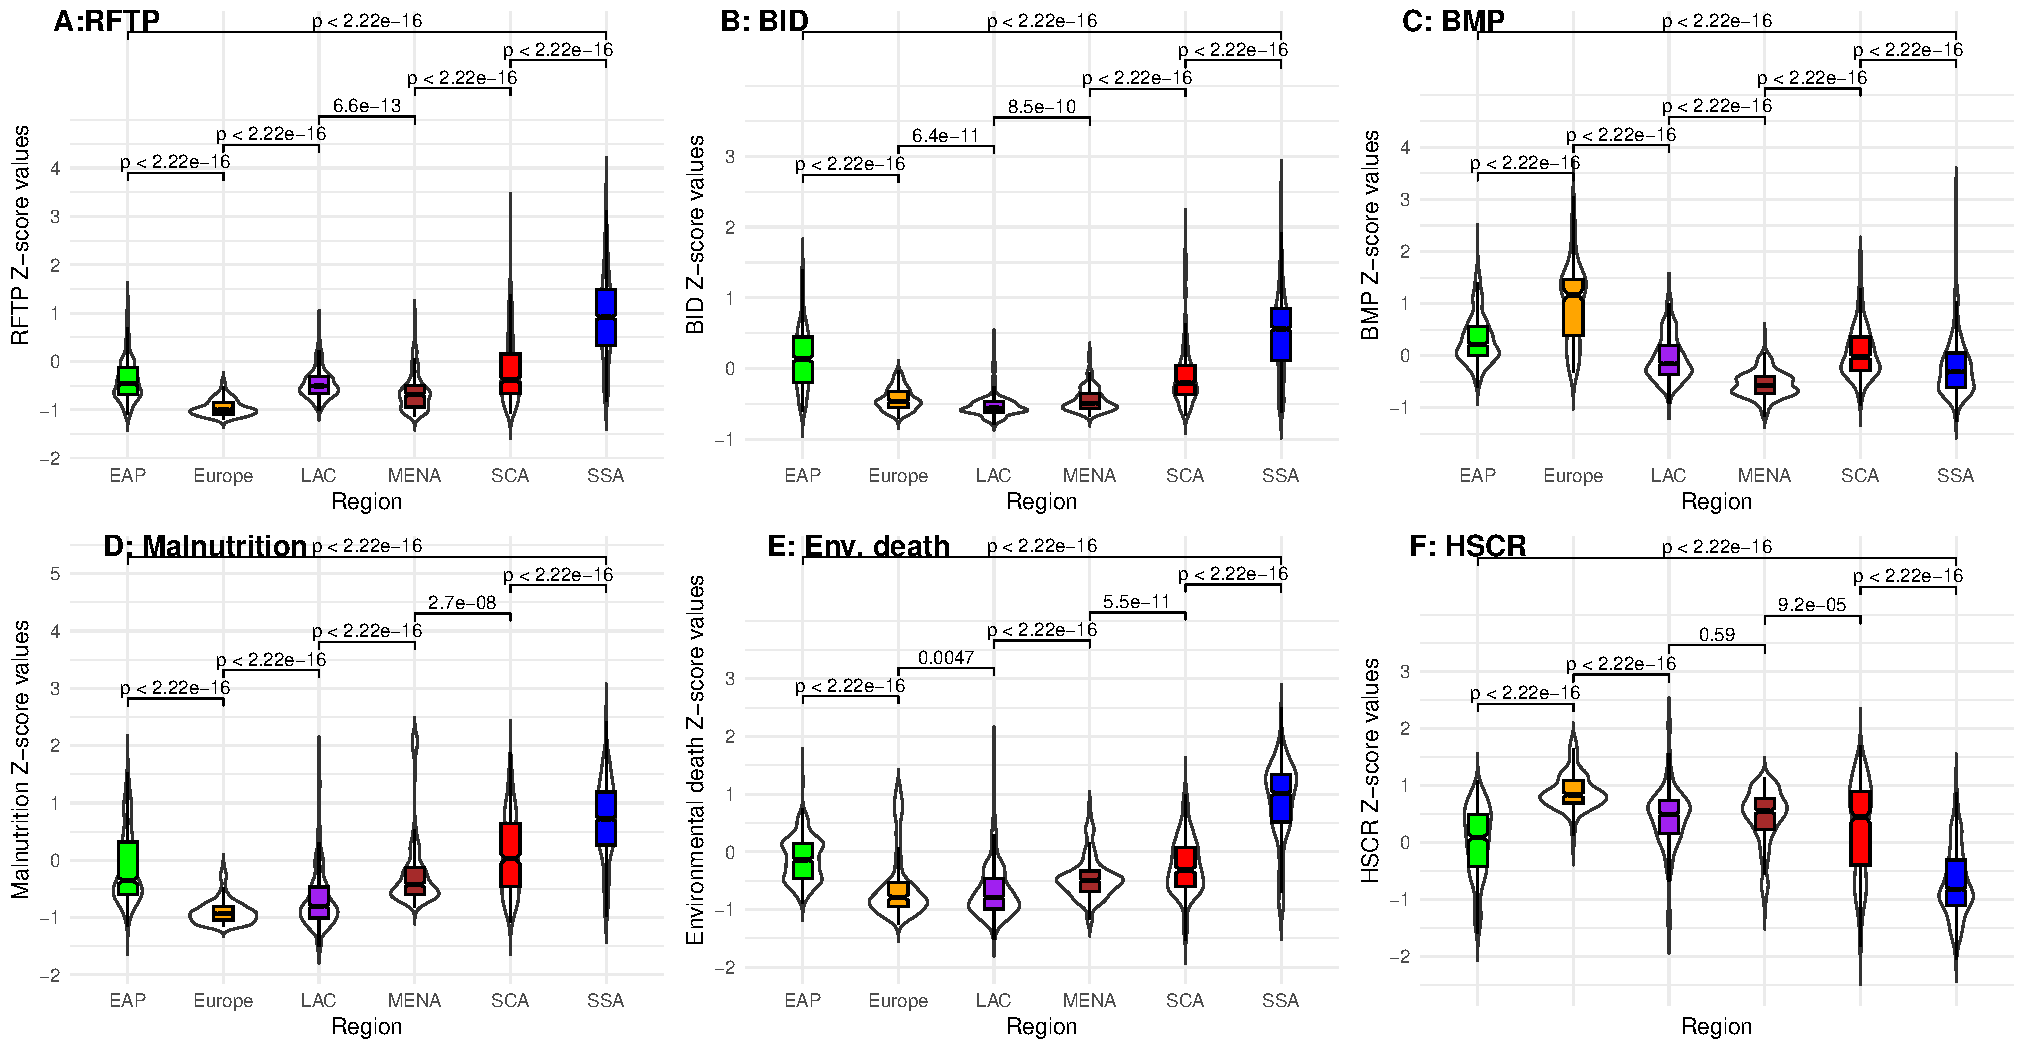
\includegraphics[width = \textwidth]{Figures and Tables/Combined_Boxplt_2.pdf}
       \caption*{\footnotesize{Note: Each plot panel corresponds to one of the six composite health dimensions, created with equal weightings.}}% Plot A features Reproductive Fatality and Teen Pregnancy (RFTP), Plot B depicts the Burden of Infection and Diseases (BID), Plot C illustrates the Burden of Mental Problems (BMP), Plot D represents Malnutrition, Plot E focuses on Environmental Death, and Plot F addresses Health System Capacity and Responsiveness (HSCR). See specific health indicators for each health dimension. Author's computation, data sourced from UNSGD (2023); WDI (2023).}}
        \end{figure}
        
\end{frame}




\begin{frame}{Conceptual Analysis Cont.: Does ODA Flow Align with Health Needs?}
    \begin{figure}
\caption{\textit{Relationship Between Total Net ODA and Health Dimensions}}
    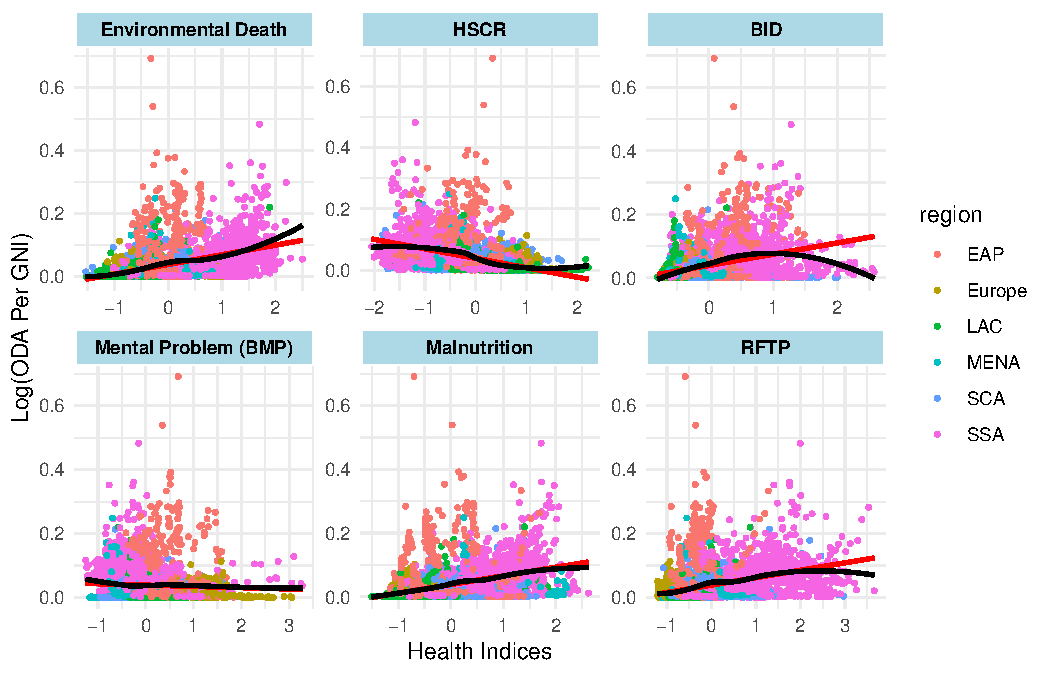
\includegraphics[width = 0.8\textwidth, height = 0.8\textheight]{Figures and Tables/ODA_Hth_plt.pdf}
    \label{fig:ODA against Hth dimension}
    %\caption*{\footnotesize{Note: Author's computation, data from UNSGD (2023); WDI (2023)}}
\end{figure}
\end{frame}



\begin{frame}{Concptual Analysis Cont.: Social Protection Roles in Health}


\begin{figure}[ht]
\caption{\textit{Relationship Between Social Protection Coverage and Health Dimensions}}
    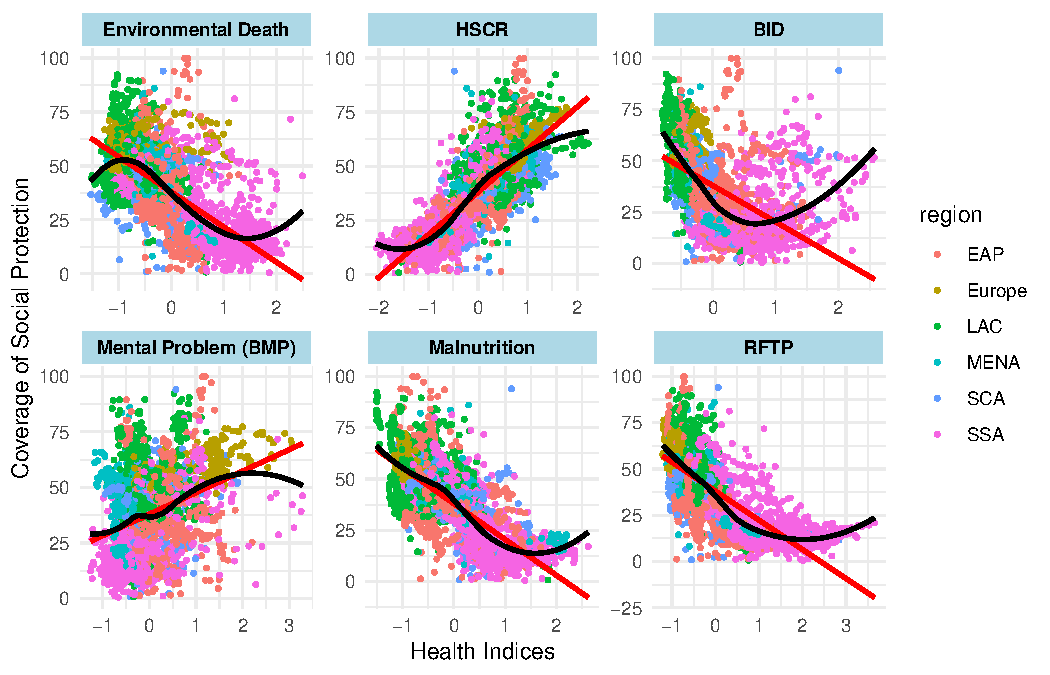
\includegraphics[width = 0.87\textwidth, , height = 0.75\textheight]{Figures and Tables/SocProct_Hlth_plt.pdf}
    \caption*{\footnotesize Note: Social protection coverage is in \% of the total population}
\end{figure}

\end{frame}



\begin{frame}{Conceptual Analysis Cont.: Major Take Away}
    In essence, the preliminary analysis chapter delves into the complex interplay between the allocation patterns of Official Development Assistance (ODA), health dimensions, and social protection.

\begin{itemize}
    \item The chapter reveals ODA allocation varies with time and reflects global situations. Moreover, Africa and Asia have been the highest recipient of ODA with the United States (US) and Germany being the highest and most predictable donors. Additionally, countries in East Asia and the Pacific (EAP) and Sub-Saharan Africa tend to be more aid-dependent than others. 
    \item By leveraging comprehensive health dimensions, the chapter unveils substantial variations in health situations across regions. Specifically, while reproductive fatality, infection and diseases, and environmental death are prevalent in SSA, SCA, and EAP, mental issue is the major problem in Europe. Moreover, Europe has the best health system capacity, with the SSA region being the poorest in the dimension. 
    \item The analysis reveals that ODA allocation does not necessarily align with the health needs of recipient countries. 
    \item Finally, While social protection tends to have a clear and discernible relationship with all health dimensions, ODA has a weak relationship with social protection. 
\end{itemize}
Note: While the preliminary offers hint on the pattern of the relationship, it does not imply causality. All hypotheses are further tested in the main analysis in Chapter Five. 
\end{frame}




\begin{frame}{Chapter Three: Theoretical Framework}
        \begin{figure}
        \caption{Figure 3: Causal chain of ODA's impact on Health outcome}
            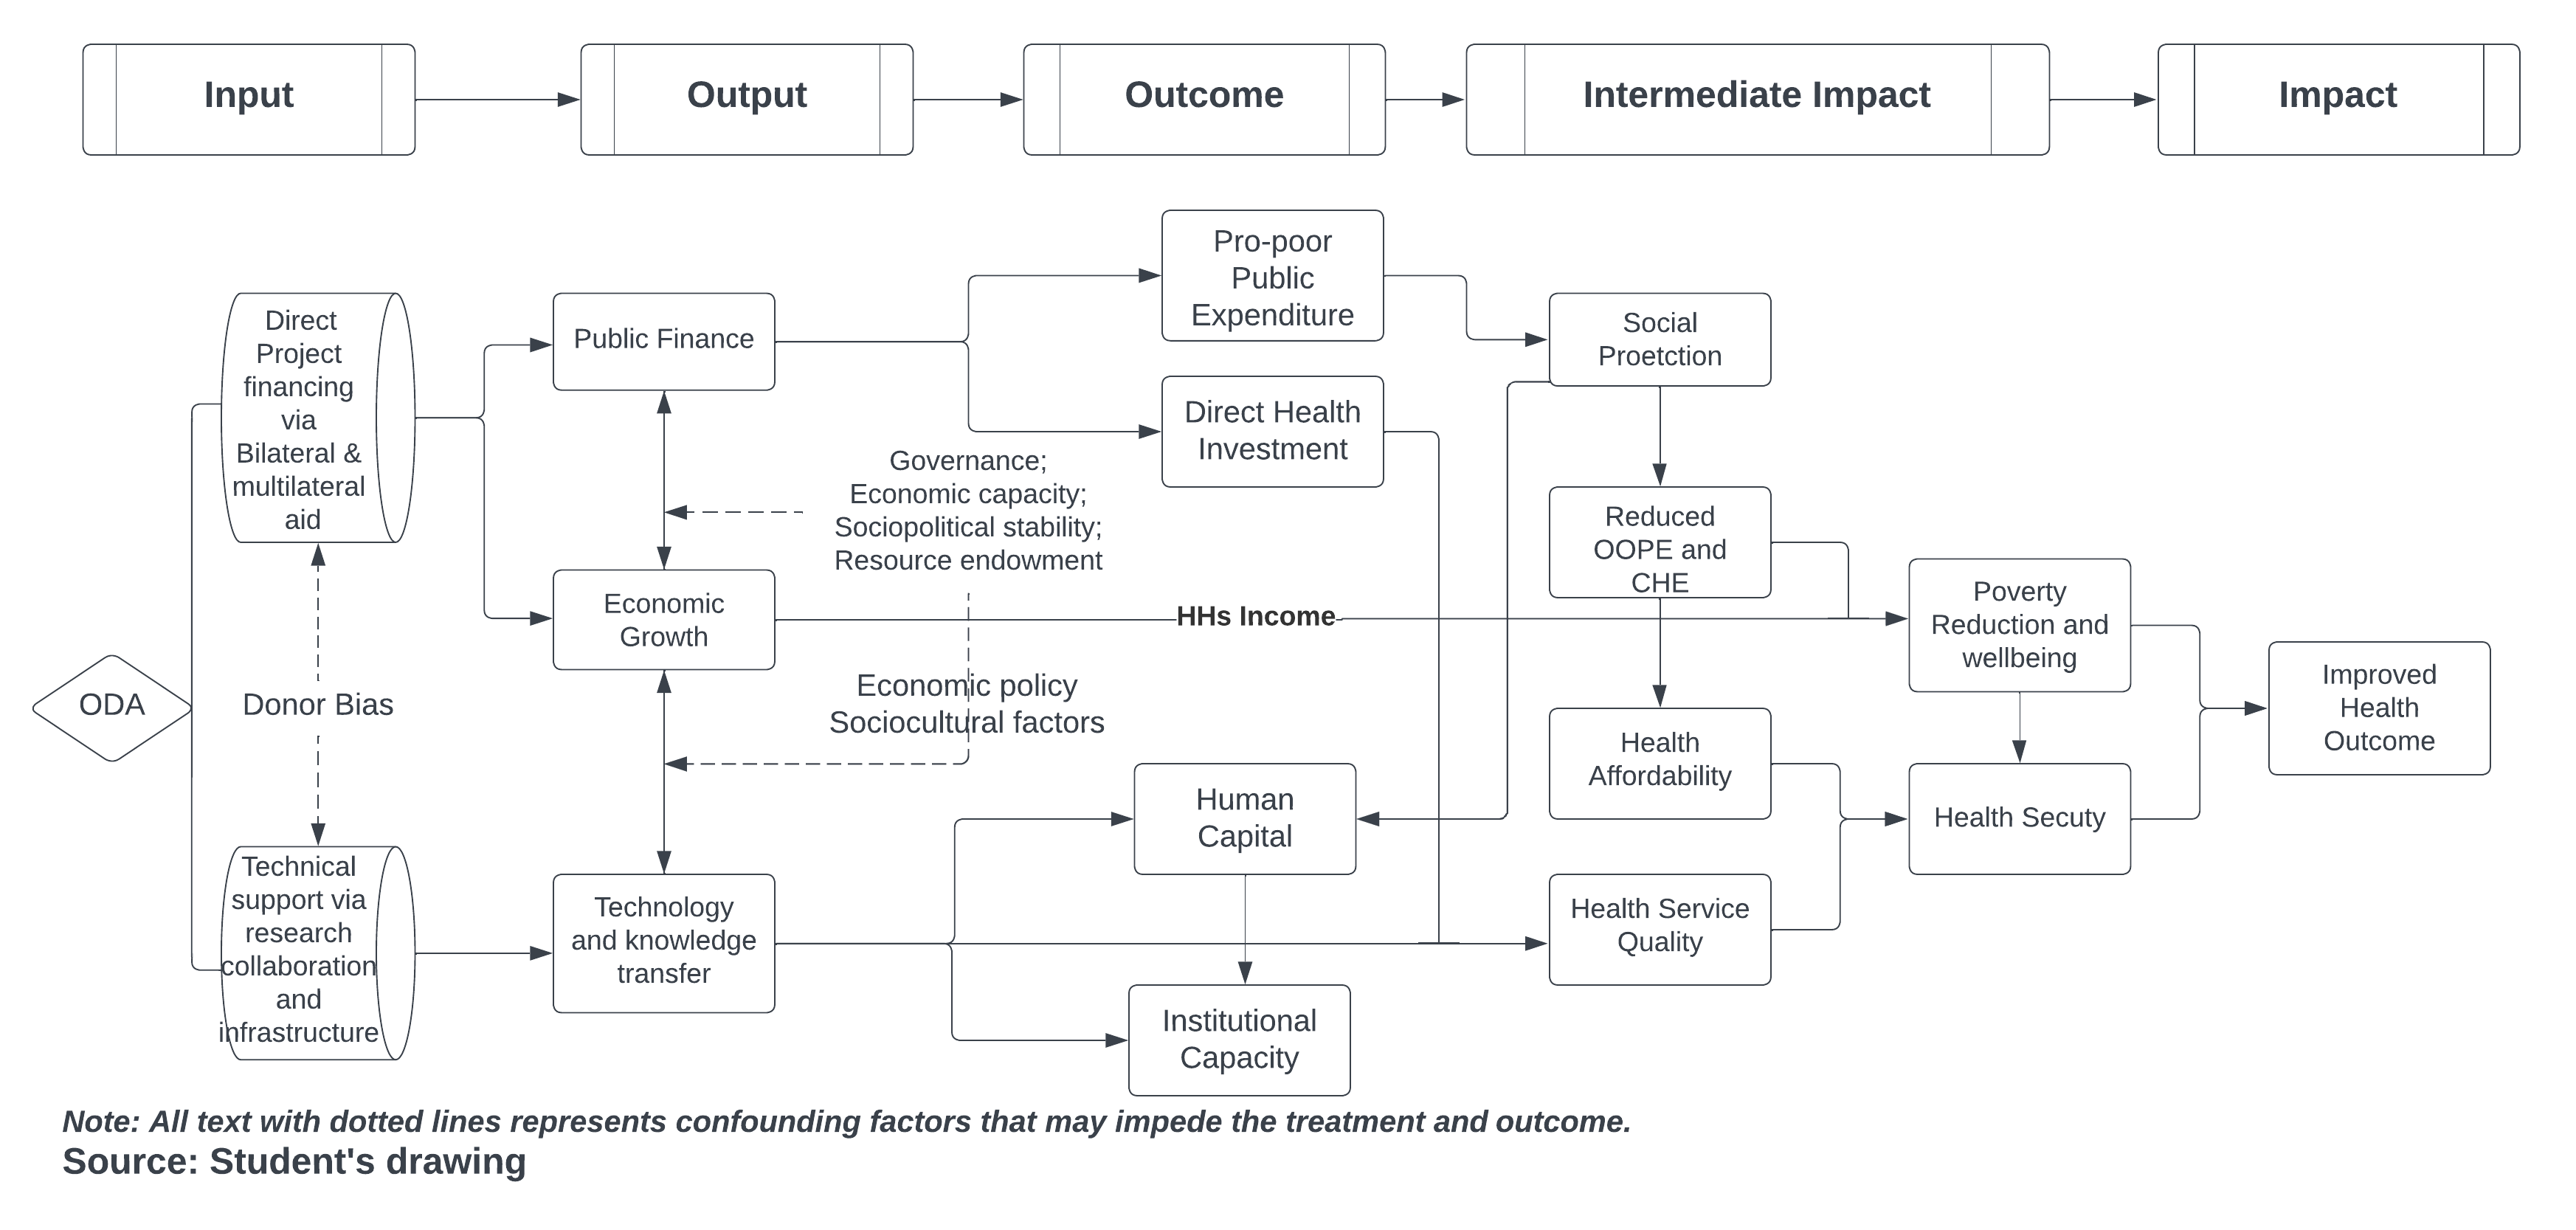
\includegraphics[width=\textwidth]{Figures and Tables/Causal Chain Graph for Thesis.png}
            
        \end{figure}
\end{frame}



\begin{frame}{Chapter Four: Research Methodology}
The study is an econometric macro-analysis, using a panel data approach. 
\begin{itemize}
    \item According to Gujarati (2004), Panel data enhances the quality of inference through: 
    \begin{enumerate}
        \item Pooling entities across different times increases the number of observations
        \item Studying behaviours across entities (countries) at different times mitigates unobserved variable bias (unobserved heterogeneity).
        \item Effective in modeling bidirectional causal relationships and sequence or predominance of the causal order.
    \end{enumerate}
\item  Panel models is categorized into static and dynamic.
\end{itemize}
In a simple static panel model, the standard assumption is that $f(y_{it}|x_{it}, \epsilon_{it})$ with $E[\epsilon | x_{it}]  = 0$:
\begin{equation}
    y_{it} = \alpha + \beta^T x_{it} + \epsilon_{it},
    \begin{cases}
        i & = 1, 2, 3, \ldots, N \\
        t & = 1, 2, 3, \ldots, T \\
    \end{cases}
    \label{eq1}
\end{equation}

Here, $\beta^T$ represents the average effect for all units (countries) $i$ at all time (year) $t$. In our context, $x$ denotes ODA allocation, while $y_{it}$ is the health outcome (HO), $\alpha$ is constant across time and units and accounts for baseline health outcome in the absence of ODA (when $x=0$).
\end{frame}



\begin{frame}{Research Methodology Cont.: Causal Assumptions}
\begin{enumerate}
    \item \textbf{Unit homogeneity and heterogeneity:} 
    \begin{itemize}
        \item Static model assumes $\beta^T$ is the same for all countries across time, thus $p(y_{it}, x_{it})$ is an ATE.
        \item Since health situations are different for countries and regions, and the impact of ODA allocation likely depends on country-level characteristics, the homogeneity assumption fails. 
        \item Failure of unit homogeneity leads to using two-way Fixed Effect in Equation \ref{eq2}:
        \begin{equation}
    HO_{it} = \beta_{1} ODA_{it} + \theta_{i} z_{it} + \mu_i + \lambda_t + \epsilon_{it}
    \label{eq2}
\end{equation}

Here, $\mu_i$ is unit time-fixed parameters for various countries, $n-1$, while $\lambda_t$ signifies the time-varying unit constant effect. $z_{it}$ is a vector of covariates.
        
    \end{itemize}
\item \textbf{Dynamic Panel Model: Reverse causality and Sequential Ignorability}
    \begin{itemize}
        \item  Fixed effect model relies on strict exogeneity, that is, past or current health conditions in a country should not directly influence the allocation of foreign aid. 
        \item This assumption is not true, as previous health conditions influence ODA allocation (feedback effect). 
        \item Moreover, ODA may also have delayed effect, that is, impact of ODA continuing till future. 
        \item As strict exogeneity fails, DPM models control for previous health outcome in Equation \ref{eq3}:
\begin{equation}
    HO_{it} = \delta_1 HO_{it-1} + \beta_{1} ODA_{it} + \theta_{i} z_{it} + \mu_i + \lambda_t + \epsilon_{it}
    \label{eq3}
\end{equation}
     
    \end{itemize}
\end{enumerate}
\end{frame}





\begin{frame}{Research Methodology Cont.: Hypotheses and Estimation Approaches}
    \textbf{Hypotheses:}
    \begin{enumerate}[i]
        \item $H_0$: \textit{The impact of ODA on all health dimensions is not significant ($\beta_{HO1} ODA_{it} = \beta_{HO2} ODA_{it} \dots \beta_{HO6} ODA_{it} = 0$}).
        \item $H_0$: \textit{The impact of ODA on health outcomes is not significantly different between SSA and non-SSA regions on at least one health dimension.}
        \item $H_0$: \textit{The indirect role of Social protection in the impact of ODA on health outcome is not statistically significant for at least one health dimension.}
    \end{enumerate}
    \textbf{Estimation Approach:}\\
\begin{itemize}
    \item Fixed Effect Cross-Lag Panel Model (FE-CLPM) (Allison et al., 2017)
    \item Unit Fixed Effect with time trend as control variable
    \item Local Projection method to understand temporal dynamics of ODA    
    \item Mediation path analysis for mediating role of social protection
\end{itemize}
\end{frame}
%%%%%%%%%%%%%%%%%%%%%%%%%%%%%%%%%%%%%%%%%%%%%%%%%%%%%%%%%%%%%%%%%%%%

\begin{frame}{Variables and Data Trasnformation}
\begin{itemize}
  \item Data 2000-2021, mean-aggregated into 5 periods, mitigating noise and serial correlation
  \item All models are estimated with mean aggregated data, except the local projection. 
\end{itemize} 
\textbf{- Variables:}
\begin{itemize}
    \item Outcome variables: health outcomes proxied by six health dimensions: reproductive fatality (RFTP), burden of infection and diseases (BID), burden of mental problem (BMP), malnutrition, environmental death, health system capacity and responsiveness (HSCR)
    \item Explanatory variables: Total net ODA (social infrastructure ODA used as robustness checks) (all log-transformed)  
    \item Control variables (Factors with competing explanatory power on health outcome) include:
    \begin{itemize}
        \item Level of development (GDP p.c., HDI)
        \item Public finance (Health spending p.c., public debt)
        \item Governance (Governance index, Bayesian Corruption Index (BCI))
        \item Infrastructure level (Access to electricity, public investment)
        \item Demographic structure (population, population density)
        \item Foreign inflow (Remittances, FDI)
        \item Climate vulnerability and exposure (Climate risk index (CRI)) 
        \end{itemize}
\end{itemize}

\end{frame}


%%%%%%%%%%%%%%%%%%%%%%%%%%%%%%%%%%%%%%%%%%%%%%%%%%%%%%%%%%%%%%%%%%%%%%%%%


\begin{frame}{Result Presentation}
\textbf{Impact of ODA on various health dimensions:}
\footnotesize
\renewcommand{\arraystretch}{0.6} 
\begin{longtable}{@{\extracolsep{5pt}}lcccccc} 
\caption{Unit Fixed Effect with Time Trend as Control (linear-log model with aggregated data)}
\\[-2ex]\hline 
\hline \\[-1ex] 
 & \multicolumn{6}{c}{\textit{Dependent variables:}} \\ 
\cline{2-7} 
\\[-1ex] 
 & RFTP & BID  & BMP & Malnutrition & ED  & HSCR \\
\\[-1.8ex] & (1) & (2) & (3) & (4) & (5) & (6)\\ 
\hline \\[-1ex]
log\_ODA\_lag       & $-0.016^{*}$   & $-0.008$       & $-0.016$       & $-0.003$       & $-0.018$       & $-0.011$      \\
Electricity                  & $-0.007^{***}$ & $-0.005^{**}$  & $-0.002$       & $-0.002$       & $-0.001$       & $0.005^{***}$ \\
log\_GDP\_Cap       & $-0.061$       & $-0.118^{*}$   & $0.027$        & $-0.495^{***}$ & $-0.233^{***}$ & $0.336^{***}$ \\
cri\_score          & $0.001$        & $0.000$        & $0.001$        & $-0.000$       & $0.001$        & $-0.001^{*}$  \\
log\_remittance     & $-0.003$       & $0.002$        & $-0.003$       & $-0.005$       & $-0.005$       & $0.007$       \\
log\_Pop            & $-1.080^{***}$ & $-0.956^{***}$ & $-0.090$       & $-0.591^{*}$   & $-0.154$       & $-0.293$      \\
log\_Pop\_dens      & $0.312$        & $0.494^{*}$    & $0.166$        & $-0.132$       & $-0.094$       & $0.501^{***}$ \\

log\_hlth\_Per\_Cap & $0.037$        & $0.031$        & $0.100^{*}$    & $-0.074$       & $0.075$        & $0.075^{*}$   \\
 Gov                 & $-0.052$       & $-0.025$       & $-0.031$       & $-0.165^{***}$ & $-0.074$       & $0.067$       \\
log\_External\_debt & $0.024$        & $0.003$        & $0.006$        & $0.035$        & $-0.026$       & $-0.036^{*}$  \\
 
time\_var           & $-0.042^{***}$ & $-0.016^{*}$   & $-0.053^{***}$ & $0.006$        & $-0.055^{***}$ & $0.024^{*}$   \\
 \hline\\
Num.Obs. & \num{576} & \num{576} & \num{576} & \num{576} & \num{576} & \num{576}\\
R2 & \num{0.768} & \num{0.566} & \num{0.258} & \num{0.621} & \num{0.564} & \num{0.581}\\
R2 Adj. & \num{0.683} & \num{0.407} & \num{-0.014} & \num{0.482} & \num{0.405} & \num{0.427}\\
AIC & \num{-1162.8} & \num{-1239.9} & \num{-872.3} & \num{-1005.1} & \num{-1006.8} & \num{-1023.8}\\
BIC & \num{-1110.6} & \num{-1187.6} & \num{-820.0} & \num{-952.8} & \num{-954.5} & \num{-971.5}\\
RMSE & \num{0.09} & \num{0.08} & \num{0.11} & \num{0.10} & \num{0.10} & \num{0.10}\\
\hline 
\hline
\textit{Note:}  & \multicolumn{3}{r}{$^{*}$p$<$0.1; $^{**}$p$<$0.05; $^{***}$p$<$0.01} \\
\label{table:FE_RQ1}
\end{longtable}


    
\end{frame}






\begin{frame}%{Impact of ODA on health dimensions cont.}

  \footnotesize
\renewcommand{\arraystretch}{0.6} 
\begin{longtable}{@{\extracolsep{3pt}}lcccccc} 
\caption{DPM: Fixed Effect Cross-Lag Panel Model (FE-CLPM) (linear-log model with aggregated data)} 
\\[-2ex]\hline 
\hline \\[-1ex] 
 & \multicolumn{6}{c}{\textit{Dependent variables:}} \\ 
\cline{2-7} 
\\[-1ex] 
 & RFTP & BID  & BMP & Malnutrition & ED  & HSCR \\
\\[-1.8ex] & (1) & (2) & (3) & (4) & (5) & (6)\\ 
\hline \\[-1ex]
log\_ODA\_lag                   & $-0.041^{***}$ & $-0.030^{**}$ & $-0.066$      & $-0.042^{**}$ & $-0.035^{*}$  & $-0.015$      \\        
ae                              & $0.000$        & $-0.001$      & $-0.003$      & $0.001$       & $0.000$       & $0.003^{***}$ \\

log\_GDP\_Cap                   & $0.062$        & $-0.010$      & $0.023$       & $-0.024$      & $0.007$       & $0.208^{***}$ \\
cri\_score                      & $-0.000$       & $-0.000$      & $-0.000$      & $-0.001$      & $0.001^{*}$   & $-0.001$      \\
log\_remittance                 & $0.000$        & $0.001$       & $0.004$       & $-0.006^{*}$  & $0.001$       & $0.005^{**}$  \\
log\_hlth\_Per\_Cap             & $-0.012$       & $-0.077$      & $-0.043$      & $0.000$       & $0.076$       & $0.094^{**}$  \\
Gov                             & $-0.053$       & $-0.001$      & $-0.001$      & $-0.063$      & $-0.043$      & $0.042$       \\
log\_External\_debt             & $0.013$        & $-0.011$      & $-0.061^{*}$  & $0.048^{*}$   & $0.010$       & $-0.021$      \\
Zscore\_Reprd\_index (t - 1)    & $0.768^{***}$  &               &               &               &               &               \\
Zscore\_InfDis\_index (t - 1)   &                & $1.138^{***}$ &               &               &               &               \\
Zscore\_Mental\_index (t - 1)   &                &               & $1.240^{***}$ &               &               &               \\

Zscore\_Nutrit\_index (t - 1)   &                &               &               & $0.896^{***}$ &               &               \\
Zscore\_EnvDeath\_index (t - 1) &                &               &               &               & $0.825^{***}$ &               \\

Zscore\_HSCR\_index (t - 1)     &                &               &               &               &               & $0.512^{***}$ \\
\hline
DF                              & $89.000$       & $89.000$      & $89.000$      & $89.000$      & $89.000$      & $89.000$      \\
Chi-Square ($\chi^2$)                           & $257.574$      & $212.063$     & $249.795$     & $286.456$     & $173.344$     & $150.279$     \\
Observations (N)                               & $144.000$      & $144.000$     & $144.000$     & $144.000$     & $144.000$     & $144.000$     \\
RMSEA                           & $0.115$        & $0.098$       & $0.112$       & $0.124$       & $0.081$       & $0.069$       \\
RMSEA  90\% CI Lower  & $0.098$       & $0.081$       & $0.096$       & $0.108$       & $0.063$       & $0.049$       \\
RMSEA  90\% CI Upper                  & $0.131$        & $0.115$       & $0.129$       & $0.140$       & $0.099$       & $0.088$       \\
p(RMSEA $<$ 0.05)                    & $0.000$        & $0.000$       & $0.000$       & $0.000$       & $0.003$       & $0.055$       \\
SRMR                            & $0.012$        & $0.015$       & $0.016$       & $0.013$       & $0.010$       & $0.006$       \\




\hline 
\hline
\textit{Note:}  & \multicolumn{3}{r}{$^{*}$p$<$0.1; $^{**}$p$<$0.05; $^{***}$p$<$0.01} \\
\label{table:FE_RQ1}
\end{longtable}


\end{frame}



\begin{frame}%{Result Presentation Cont.: Impact of ODA on Health Dimensions}
\textbf{- Local Projections: Understanding the Temporal Dynamics of ODA Impact on Health}
\begin{equation}
HO_{it + h} = \beta^h ODA_{it} + \theta z_{it} + \mu_{i} + \lambda_{t} + \epsilon_{it}
\label{eq::local_projection}
\end{equation}
    \begin{figure}
        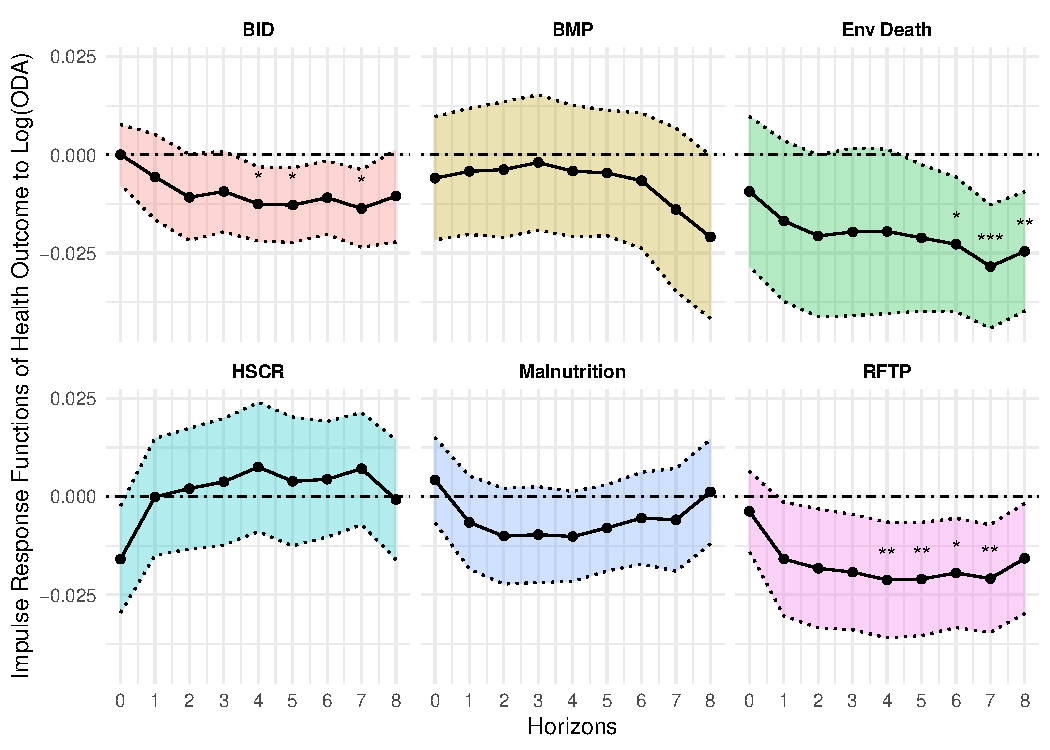
\includegraphics[width= 0.9\textwidth, height = 0.87\textheight]{Figures and Tables/Local_Projt.pdf}
        \end{figure}
\end{frame}





\begin{frame}{Result Presentation Cont.: Regional Variation of ODA Impact}
Note: All covariates have been removed to prevent too long table
\footnotesize
\renewcommand{\arraystretch}{0.6} 
\begin{longtable}{@{\extracolsep{5pt}}lcccccc} 
\caption{Unit Fixed Effect with Time Trend as Control (linear-log model with aggregated data)}
\\[-2ex]
\hline 
\hline \\[-1ex] 
 & \multicolumn{6}{c}{\textit{Dependent variables:}} \\ 
\cline{2-7} 
\\[-1ex] 
 & RFTP & BID  & BMP & Malnutrition & ED  & HSCR \\
\\[-1.8ex] & (1) & (2) & (3) & (4) & (5) & (6)\\ 
\hline \\[-1ex]

EAP\_log\_ODA\_lag             & $0.013$        & $-0.007$       & $0.001$      & $-0.003$       & $0.001$        & $-0.001$      \\
SSA\_dum:log\_ODA\_lag    & $-0.005$       & $-0.004$       & $-0.020$     & $0.021$        & $0.010$        & $0.006$       \\
MENA\_dum:log\_ODA\_lag   & $-0.027^{*}$   & $0.032^{**}$   & $-0.011$     & $0.002$        & $0.019$        & $0.011$       \\
LAC\_dum:log\_ODA\_lag    & $-0.004$       & $0.010$        & $-0.010$     & $-0.003$       & $-0.002$       & $-0.008$      \\
SCA\_dum:log\_ODA\_lag    & $-0.022$       & $0.026$        & $0.003$      & $0.030$        & $0.000$        & $0.037$       \\

Europe\_dum:log\_ODA\_lag & $-0.032^{**}$  & $-0.009$       & $-0.016$     & $0.002$        & $-0.041^{*}$   & $-0.009$      \\

\hline
\midrule
Num.Obs. & \num{576} & \num{576} & \num{576} & \num{576} & \num{576} & \num{576}\\
R2 & \num{0.801} & \num{0.651} & \num{0.355} & \num{0.587} & \num{0.559} & \num{0.617}\\
R2 Adj. & \num{0.725} & \num{0.518} & \num{0.108} & \num{0.429} & \num{0.391} & \num{0.471}\\
AIC & \num{-1820.2} & \num{-1615.0} & \num{-1488.1} & \num{-1751.1} & \num{-1725.0} & \num{-1894.8}\\
BIC & \num{-1746.1} & \num{-1540.9} & \num{-1414.0} & \num{-1677.0} & \num{-1650.9} & \num{-1820.7}\\
RMSE & \num{0.05} & \num{0.06} & \num{0.06} & \num{0.05} & \num{0.05} & \num{0.05}\\

\hline 
\hline
\textit{Note:}  & \multicolumn{3}{r}{$^{*}$p$<$0.1; $^{**}$p$<$0.05; $^{***}$p$<$0.01} \\
\label{table:FE_RQ1}
\end{longtable}
 
\end{frame}







\begin{frame}{Result Presentation Cont.: Regional Variation of ODA Impact}

\footnotesize
\renewcommand{\arraystretch}{0.6} 
\begin{longtable}{@{\extracolsep{5pt}}lcccccc} 
\caption{DPM: Regional Heterogeneity with FE-CLPM (linear-log model with aggregated data)}
\\[-2ex]\hline 
\hline \\[-1ex] 
 & \multicolumn{6}{c}{\textit{Dependent variables:}} \\ 
\cline{2-7} 
\\[-1ex] 
 & RFTP & BID  & BMP & Malnutrition & ED  & HSCR \\
\\[-1.8ex] & (1) & (2) & (3) & (4) & (5) & (6)\\ 
\hline \\[-1ex]
EAP\_log\_ODA\_lag                   & $0.005$       & $-0.030$      & $-0.001$      & $-0.041$      & $0.004$       & $0.006$       \\
 SA\_ODA                        & $-0.051$      & $-0.035$      & $-0.043$      & $0.096^{*}$   & $-0.030$      & $0.031$       \\
 ENA\_ODA                       & $-0.011$      & $0.061$       & $0.023$       & $0.037$       & $0.011$       & $-0.020$      \\
  
LAC\_ODA                        & $0.192^{**}$  & $-0.217^{**}$ & $-0.422^{*}$  & $-0.213^{**}$ & $0.264^{**}$  & $-0.284^{**}$ \\
  
SCA\_ODA                        & $-0.056$      & $-0.088$      & $-0.068$      & $0.239^{***}$ & $-0.008$      & $-0.102$      \\
  
Europe\_ODA                     & $-0.037$      & $0.031$       & $-0.008$      & $0.058$       & $-0.068^{*}$  & $-0.005$      \\
Autoregressive Parameter   & $0.770^{***}$ &     $0.953^{***}$          &    $0.987^{***}$           &    $0.829^{***}$           &     $0.737^{***}$          &        $0.783^{***}$       \\
                                & $(0.043)$     & $(0.093)$       &  $(0.100)$             &       $(0.096)$        &       $(0.121)$        &    $(0.112)$           \\
                                
 \hline\\
DF                              & $125.000$     & $125.000$     & $125.000$     & $125.000$     & $125.000$     & $125.000$     \\
Chi-square ($\chi^2$)                           & $280.205$     & $211.046$     & $233.490$     & $259.328$     & $184.373$     & $193.121$     \\
Observation (N)                               & $144.000$     & $144.000$     & $144.000$     & $144.000$     & $144.000$     & $144.000$     \\
RMSEA                           & $0.093$       & $0.069$       & $0.078$       & $0.086$       & $0.057$       & $0.062$       \\
RMSEA 90\% CI Lower                  & $0.078$       & $0.053$       & $0.062$       & $0.071$       & $0.039$       & $0.044$       \\
RMSEA 90\% CI Upper                  & $0.107$       & $0.085$       & $0.093$       & $0.101$       & $0.074$       & $0.078$       \\
p(RMSEA $<$ 0.05)             & $0.000$       & $0.030$       & $0.003$       & $0.000$       & $0.238$       & $0.134$       \\
SRMR                            & $0.007$       & $0.011$       & $0.011$       & $0.008$       & $0.009$       & $0.009$       \\
\hline 
\hline
\textit{Note:}  & \multicolumn{3}{r}{$^{*}$p$<$0.1; $^{**}$p$<$0.05; $^{***}$p$<$0.01} \\
\label{table:FE_RQ1}
\end{longtable}


    
\end{frame}






\begin{frame}{Result Presentation Cont.: Mediation Analysis of Social Protection in ODA Impact}
   \renewcommand{\arraystretch}{0.85} % 
   
\footnotesize
\renewcommand{\arraystretch}{0.6} 
\begin{longtable}{@{\extracolsep{5pt}}lcccccc} 
\caption{Mediation Analysis of Social Protection in ODA impact on Health Outcomes (linear-log model)}
\\[-2ex]\hline 
\hline \\[-1ex] 
 & \multicolumn{6}{c}{\textbf{Main Predictor: log(ODA)$_{it-4}$}} \\
 & & & & & & \\ 
 & \multicolumn{6}{c}{\textbf{Mediating Variable: Social\_Protection\_Coverage$_{it-3}$}} \\
\cline{2-7} 
\\[-1.8ex] & \multicolumn{6}{c}{ } \\ 
 & Reproductive & Malnutrition  & Infections and & Health & Envir. & Mental\\
 & Fatalities & & Diseases & Capacity & Death & Burden \\
\\[-1.8ex] & (1) & (2) & (3) & (4) & (5) & (6)\\ 
\hline \\[-1ex] 
\textbf{Total Effect}: & $-$0.008$^{***}$ & $-$0.015 &$-$0.002 & 0.031 & $-$0.006 & 0.026 \\
 & (0.002)& (0.020)& (0.002)& (0.025) & (0.015)& (0.016)\\
 & & & & & & \\ 
 \textbf{Direct Effect}: & $-$0.008$^{***}$ & $-$0.015 & $-$0.002 & 0.031 & $-$0.006 & 0.026\\
 & (0.002) & (0.020) & (0.002) & (0.025) & (0.015)&  (0.016)\\
 & & & & & & \\  
 \textbf{Indirect Effect}: & $-$0.000 & 0.000 & $-$0.000 & $-$0.000 & 0.000 & $-$0.000\\
 \textbf{Lower CI}: & $-$0.00010 &$-$0.00253 &  $-$0.00005 & $-$0.00245  &  $-$0.00217 & $-$0.00060\\ 
\textbf{Upper CI}: & 0.00006 & 0.00258 & 0.00004 & 0.00218 & 0.00249 & 0.000347 \\
 & & & & & & \\ 
\hline \\[-1ex] 
Confidence Level: & 95\% & 95\% & 95\% & 95\% & 95\% & 95\%\\
Bootstrap &&&&&& \\
Replicates: & 5000 & 5000 & 5000 & 5000 & 5000 & 5000\\
\bottomrule
\hline \\[-1ex] 
\textit{Note:}  & \multicolumn{6}{r}{$^{*}$p$<$0.1; $^{**}$p$<$0.05; $^{***}$p$<$0.01} \\ 

\end{longtable}  
\end{frame}


\begin{frame}{Insights from findings}
The impact of foreign aid (ODA) on health varies based on ODA type, econometric model, and health dimensions. Despite the mix findings, the study reveals the followings insights:  
\begin{enumerate}
    \item ODA Impact on Health:
\begin{itemize}
    \item Both total and social infrastructure ODA have positive impacts on reproductive fatality, infections and diseases, as well as environmental death across multiple models.
    \item Surprisingly, all coefficients of ODA for health system capacity (HSCR) are negative.
    \item Temporal dynamics of ODA impact: using year-wave data show intermediate (4 years) and long-term (6 years) effects of ODA on reproductive fatalities and infections and diseases, while ODA's impact on environmental death is long-term.
\end{itemize}
    
    \item Regional Heterogeneity:
\begin{itemize}
    \item Weak evidence suggests varying impacts of ODA on health across Sub-Saharan Africa (SSA) and non-SSA regions, with social infrastructure ODA more impactful on reproductive fatality in SSA, EAP, and MENA regions.
    \item Social infrastructure ODA is only significant for health system capacity in the EAP region.
\end{itemize}
    
    \item Mediating Role of Social Protection in the ODA Impact
    \begin{itemize}
        \item There is no evidence that social protection plays an indirect role in ODA's impact on health.
        \item Due to data limitations and causal order assumptions, findings are presented as a pragmatic policy guide rather than definitive conclusions.
    \end{itemize}
\end{enumerate}    
\end{frame}




\begin{frame}{Conclusions:}

\begin{itemize}
    \item While there is evidence that ODA has an impact on various health problems, there is no evidence that ODA enhances health system capacity, which is crucial to ensuring sustainable health security in developing countries.
    \item This is perhaps why William Easterly argued ODA focuses on treatment rather than prevention (Easterly, 2004)
    \item This study contributes to the pool of evidence on the effectiveness of foreign aid. However, it is important to acknowledge certain limitations, including the causal assumption, data quality, and model specifications, that may have influenced the results.
    \item In essence, no study has the best model, as threats to validity can only be mitigated, not eliminated. 
    \item Thus, the true causal impact of ODA on health lies at the confluence of many evidence, including the previous studies. 
 
\end{itemize}    
\end{frame}



\begin{frame}{Policy Recommendations}
\begin{itemize}
    \item \textbf{ODA Allocation Mechanisms Strengthening:}
        \begin{itemize}
            \item Preliminary findings suggest ODA allocation patterns do not align with countries' health needs.
            \item Strengthening the capacity of the Development Assistance Committee (DAC) of the OECD and implementing a result-based financing approach can enhance targeted ODA allocation.
        \end{itemize}
    
    \item \textbf{Optimal Utilization of ODA by Recipient Governments:}
        \begin{itemize}
            \item Recipient governments should adopt a visionary approach to ODA utilization.
            \item Prioritize policies enhancing healthcare systems, poverty alleviation, and investments in education, social protection, and health research to build absorptive capacity and optimize ODA effectiveness.
        \end{itemize}
    
    \item \textbf{Governance and Accountability:}
        \begin{itemize}
            \item Governance deficiencies, such as corruption, impede ODA effectiveness.
            \item Propose international sanctions for governments mismanaging ODA, including prevention from future access or requests for ODA return, to enhance accountability.
        \end{itemize}
    
    \item \textbf{Focus on Economic Development, Debt Forgiveness, and Conflict Prevention:}
        \begin{itemize}
            \item Economic development and excessive debt contribute to poverty and poor health outcomes.
            \item The International community should prioritize development efforts on critical health infrastructures that boost health systems, and debt forgiveness, as well as preventing war and violence in developing countries.
        \end{itemize}
\end{itemize}
\end{frame}





\newgeometry{margin = 0pt}
%%%%%%%%%%%%%%%%%%%%%%%%%%%%%%%%%%%%%%%%%%%%%%%%%%%%%%%%%%%%%%
% Slide 1: Title Page

\begin{frame}[noframenumbering,plain]
\vspace{9pt}
  \begin{figure}
\fullframegraphic{
\includegraphics[width= \paperwidth, height = \paperheight]{Final_slide.pdf}}
       \end{figure}
\end{frame}

%%%%%%%%%%%%%%%%%%%%%%%%%%%%%%%%%%%%%%%%%%%%%%%%%%%%%%%%%%%%
\restoregeometry




\end{document}